\chapter{Testing and Evaluation}

\section{Testing}

Software testing is an investigation conducted to provide information about the quality of the product or service under test. Testing is executing a system in order to identify any gaps, errors, or missing requirements in contrary to the actual requirements. In my project I am using test-driven approach method, this helps eliminate parts of the code that will not work or fix them before adding them to system.

\subsection{Service testing}

As this project is Test Driven Development approach, all service unit testing has previously been done. These tests were done by building a small client application in Playground and web-server in Perfect which was developed and ran in Xcode. The API requests were tested afterwards using the Postman application, to run each API request and ensure the result is as expected. The tested included check the secret key and application key were authenticated, and if an incorrect key was used, then an error would be returned. Included bottom are some of the requests made along with the response in table \ref{tb:service-testing}.

\begin{table}[!h]
\centering
\caption{Service Testing}
\label{tb:service-testing}
\begin{tabular}{|c|c|c|l|l|}
\hline
\rowcolor{green!20}
\multicolumn{1}{|l|}{API Call}  & \multicolumn{1}{l|}{HTTP method} & \multicolumn{1}{l|}{Response}   & Body    & Result \\ \hline
\begin{tabular}[c]{@{}c@{}}http://perfectserver.site/api/\\ cc2b14fa-f59b-4e13-905a-3eebaf2ff659/\\ storage/RemoteConfig\end{tabular} & GET                                                      & Figure \ref{fig:api1}                                                                                                            &                                                                                                                                                     & PASS                           \\ \hline
\begin{tabular}[c]{@{}c@{}}http://perfectserver.site/\\ storage/TBAnalyitcs/\end{tabular}                                             & GET                                                      & \begin{tabular}[c]{@{}c@{}}\{,"result": "error"\\ ,"message": ""\}\end{tabular}                                             &                                                                                                                                                     & FAIL                           \\ \hline
\begin{tabular}[c]{@{}c@{}}http://perfectserver.site/api/\\ cc2b14fa-f59b-4e13-905a-3eebaf2ff659/\\ storage/Friends\end{tabular}      & GET                                                      & Figure \ref{fig:api2}                                                                                                            &                                                                                                                                                     & PASS                           \\ \hline
\begin{tabular}[c]{@{}c@{}}http://perfectserver.site/api/\\ cc2b14fa-f59b-4e13-905a-3eebaf2ff659/\\ storage/Friends\end{tabular}      & POST                                                     & \begin{tabular}[c]{@{}c@{}}\{,"result": "success",\\ "message":\\  "0e9635f6-b3fd-408d-\\ b4a2-458dab34c781"\}\end{tabular} & \begin{tabular}[c]{@{}l@{}}\{"dob": "12/12/2016",\\ "age": "44",\\ "name": "Jimmy"\\ ,"county": "Portsmouth"\\ ,"country": "England"\}\end{tabular} & \multicolumn{1}{c|}{PASS}      \\ \hline
\end{tabular}
\end{table}

\begin{figure}[!h]
    \caption{API Call 1}
    \centering
    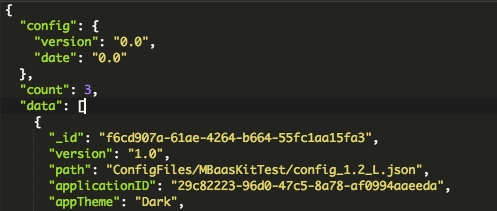
\includegraphics[width=100mm]{images/testing/api1}
    \label{fig:api1}
\end{figure} 

\begin{figure}[!h]
    \caption{API Call 2}
    \centering
    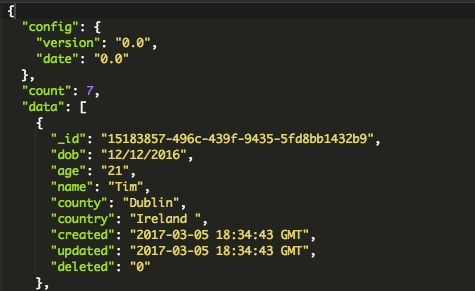
\includegraphics[width=100mm]{images/testing/api2}
    \label{fig:api2}
\end{figure} 

\newpage

\subsection{Integrated App Testing}

This part of testing involved developing a new mobile application with a simply user interface. The SDK developed was downloaded uses Cocoapods and installed in the testing app workspace. The application illustrated in the following figures \ref{fig:dark-theme} and \ref{fig:light-theme} , displays a table view where an array of "Friends" are displayed. The objective of created this test application is to demonstrate the remote configuration that allows the user to choose a new theme \ref{fig:app-themes-options} , and instantly see the difference.

The project aim from the beginning was to speed up development, testing and when the app is live. The figures \ref{fig:dark-theme} and \ref{fig:light-theme} illustrates how the app can be updated when the application is live quickly. The next three listings illustrate on what is required in the development stage to be able to update the UI objects when the app is published. 

In listing \ref{lst:test1} is UI objects include label and button, and these in one line can be initialised to start using the remote configuration feature.

\lstinputlisting[label={lst:test1},language=Swift, caption=Remote Config demo1]{testing_evaluation/code/test_project1.m}

In listing \ref{lst:test2} illustrates how the remote configuration file is being retrieved based on the theme chosen.

\lstinputlisting[label={lst:test2},language=Swift, caption=Remote Config demo2]{testing_evaluation/code/test_theme.m}

In listing \ref{lst:test2} the configuration file is being updated. This mean the old file is being deleted, and the new file updated to current main name and location. Next the navigation bar is being updated.

\lstinputlisting[label={lst:test3},language=Swift, caption=Remote Config demo3]{testing_evaluation/code/test_update.m}

\begin{figure}[!h]
    \caption{App Theme options}
    \centering
    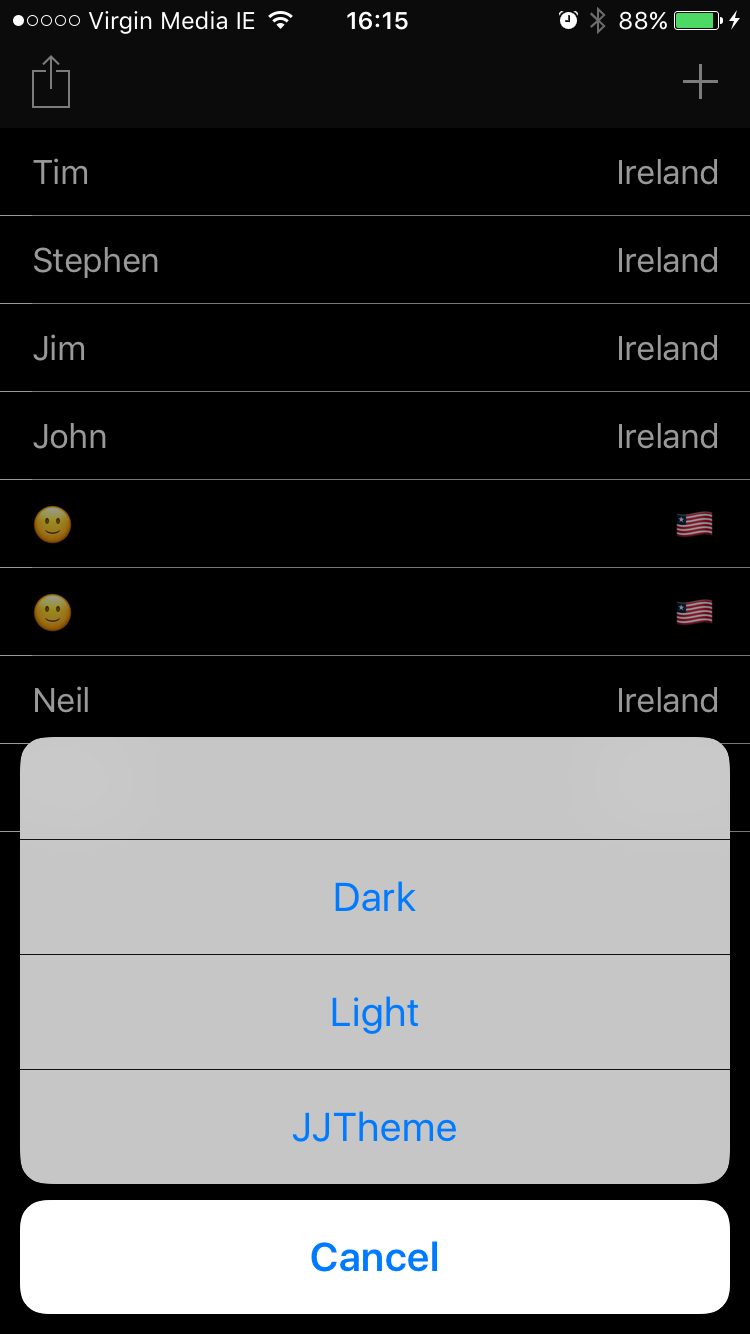
\includegraphics[width=60mm]{images/testing/themes}
    \label{fig:app-themes-options}
\end{figure} 

\begin{figure}[!h]
    \begin{subfigure}{0.5\textwidth}
        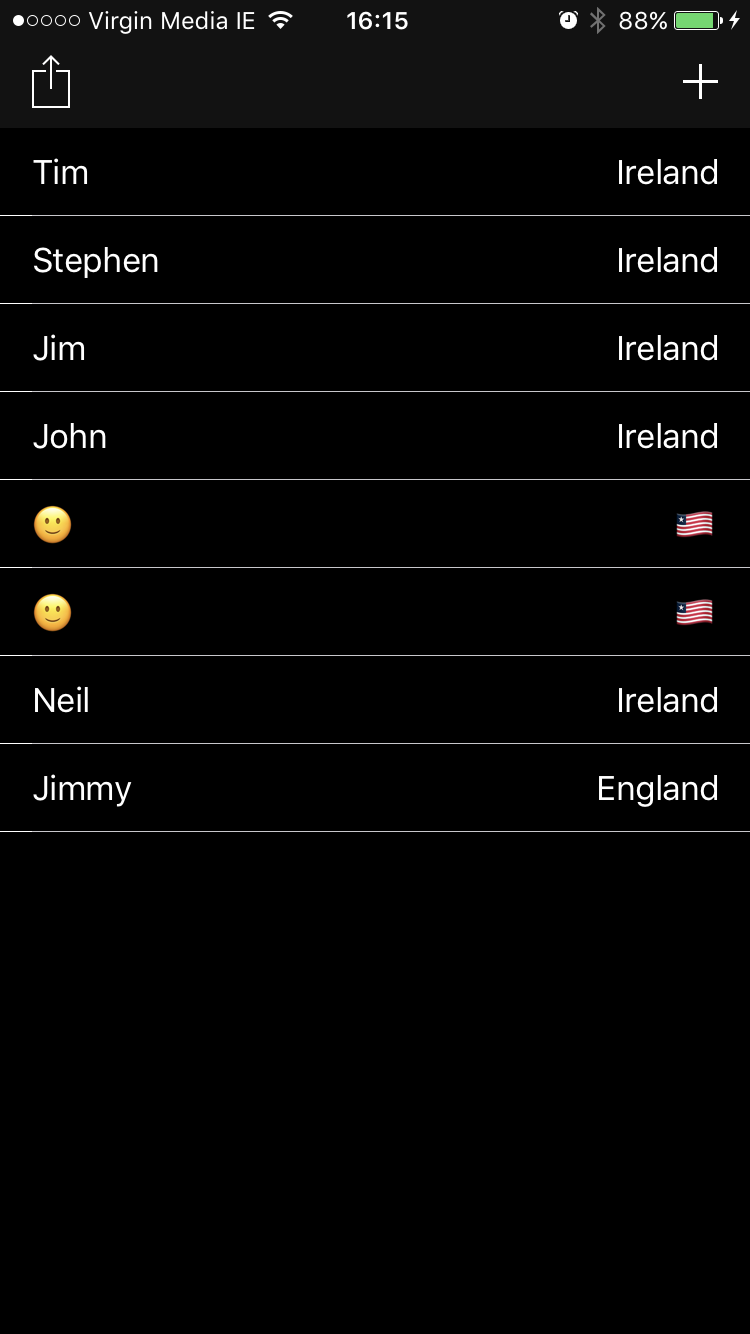
\includegraphics[width=0.8\linewidth, height=9cm]{images/testing/darkTheme}
        \caption{Dark Theme}
        \label{fig:dark-theme}
    \end{subfigure}
    \begin{subfigure}{0.5\textwidth}
        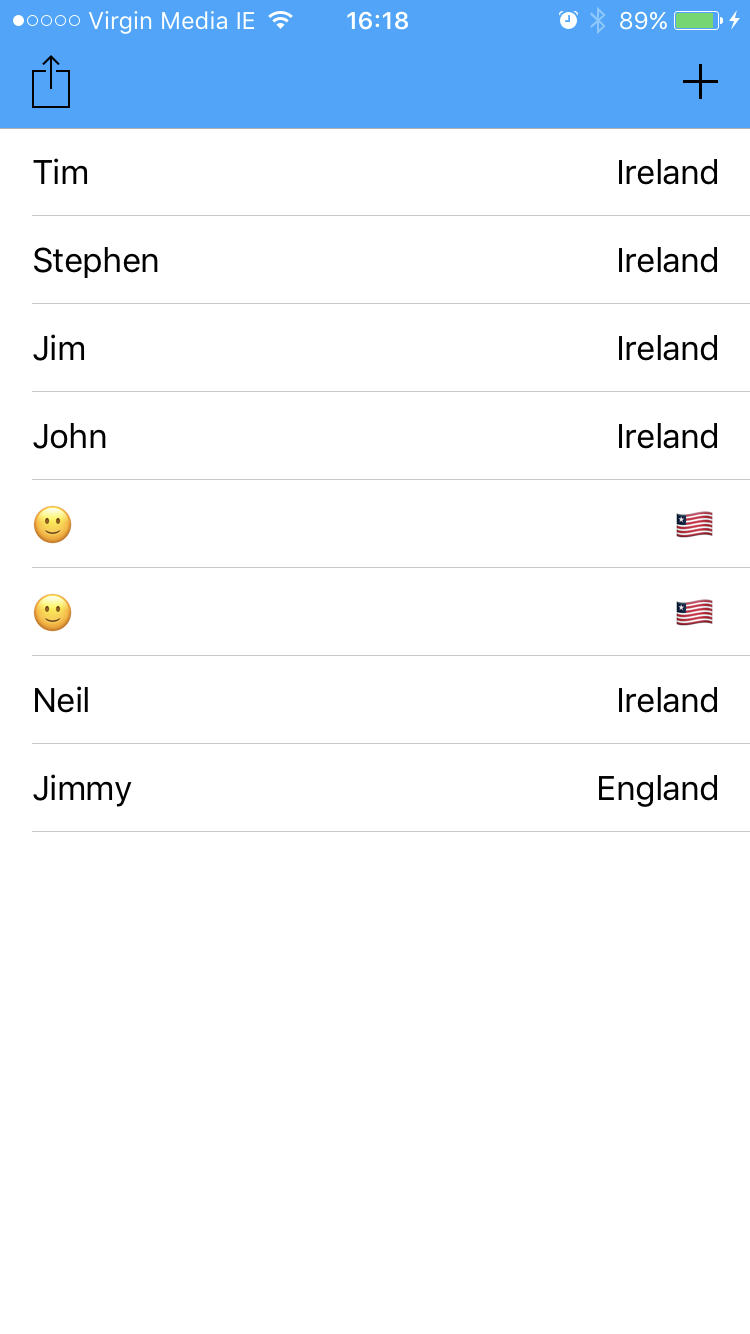
\includegraphics[width=0.8\linewidth, height=9cm]{images/testing/lightTheme}
        \caption{App Version}
        \label{fig:light-theme}
    \end{subfigure}
\caption{App Themes}
\label{fig:app-themes}
\end{figure}


\subsection{User testing}

\section{Evaluation}

